%
% Dataontwerp
%

\chapter{Dataontwerp}

\begin{figure}[h!]
	\centering
		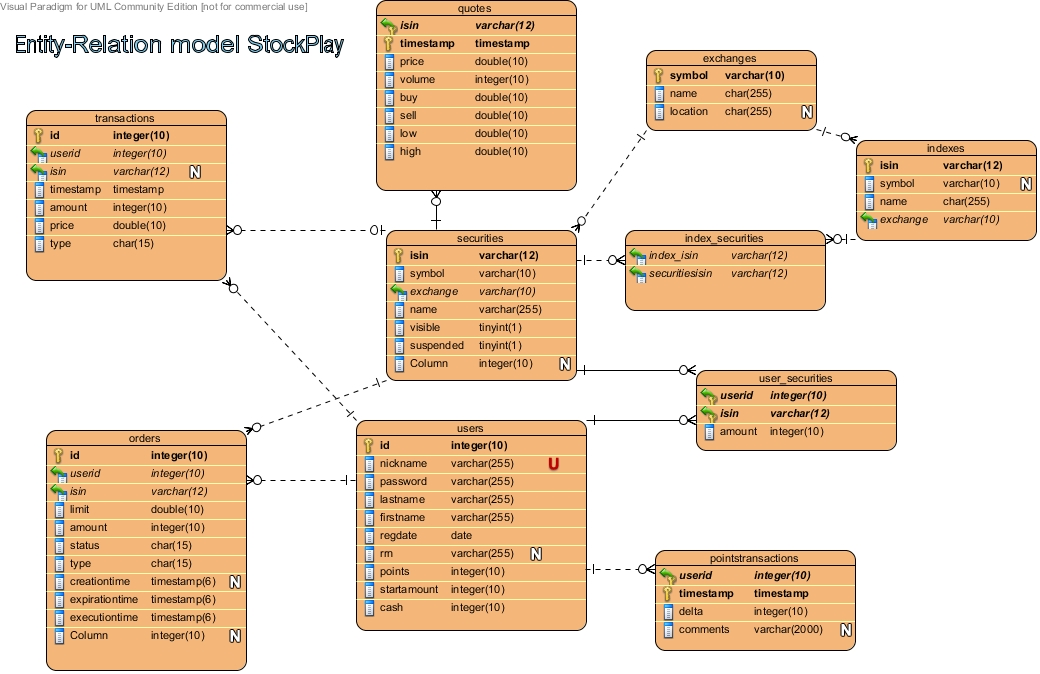
\includegraphics[width=0.5\textwidth]{images/realisatie/ER_Diagram}
	\caption{Entity-relationship model.}
\end{figure}

\section{Ontwerp backend}
\todo{dit hoort hier niet}
De klassen die de persistente data uit de database moeten weergeven staan opgesomd in onderstaand klassendiagram:

\begin{figure}[h!]
	\centering
		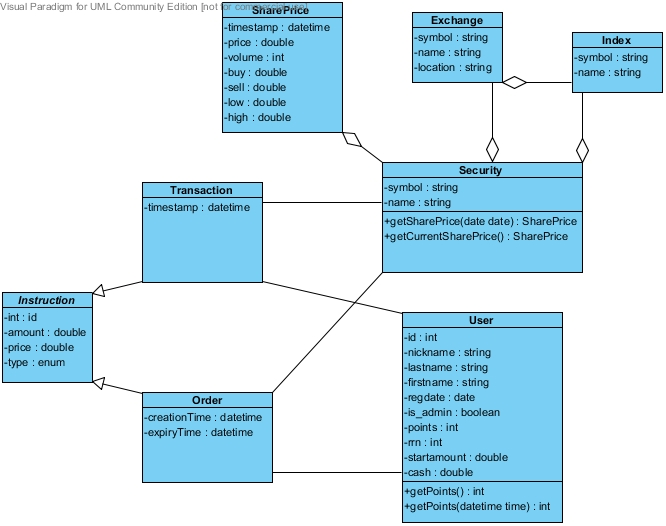
\includegraphics[width=0.5\textwidth]{images/realisatie/Class_Diagram}
	\caption{Klassendiagram persistente data in backend.}
\end{figure}

Op onze databank hebben we ook een aantal triggers. De punten mogen niet zomaar mogen aangepast in de gebruikerstabel. Elke wijziging gebeurt via de pointshistory tabel. Het toevoegen van een nieuw record daarin zorgt ervoor dat een trigger de delta waarde in de pointshistory optelt bij de punten in de userstabel. Zodoende hebben we een cache van het puntentotaal die we snel kunnen raadplegen.

Ook bij het omzetten van een order naar een transactie wordt een trigger geactiveerd die nakijkt of de gebruiker wel voldoende cash positie bezit.

De cash positie van een gebruiker kan niet zomaar aangepast worden, dit wordt ook beveiligd met een trigger.


%
% Procedureontwerp
%

\chapter{Procedureontwerp}

\section{XML-RPC interface}

Zoals vermeld bij het technisch ontwerp, gebruiken we het XML-RPC protocol als communicatiemiddel tussen de backend en zijn interfaces. Hiertoe moeten we de set aan functies vastleggen die een client kan uitvoeren, en de bijhorende signatuur documenteren.

Aangezien XML-RPC geen ondersteuning biedt voor namespaces of andere vormen van functieorganisatie, hanteren we zelf een mechanisme om dit te bekomen: een methode-naam bestaat altijd uit twee delen, gescheiden door een punt. Het deel voor het scheidingsteken duidt het pakket aan, het deel erna de methode die we willen oproepen.
Zo delen we de backend op in de volgende drie primaire klassen:
\begin{itemize}
\item{System: functionaliteit voor beheer en de statusinformatie van het systeem.}
\item{User: beheer van gebruikers en ophalen gebruikersinformatie.}
\item{Finance: functionaliteit gerelateerd aan het beurswezen.}
\end{itemize}
Hogere-orde klassen zijn eventueel ook mogelijk (zoals \emph{System.Database}), maar niet verplicht. De semantiek is daarbij identiek aan primaire klassen, met een punt als scheidingsteken.

\subsection{Algemene foutcodes}

De XML-RPC specificatie biedt ook ondersteuning voor foutberichten, in de form van een bericht met een $<$fault$>$ tag. Die tag moet steeds twee $<$member$>$ tags bevatten, namelijk een foutcode $<$faultCode$>$ van het integer type, en een foutbericht $<$faultString$>$ van het string type. Elk van de klassen kan zo specifieke foutmeldingen vastleggen.
Maar er zijn ook generieke foutmeldingen, die van toepassing zijn op alle klassen. Deze foutmeldingen, waarvan de foutcode in het bereik $[0, 100[$ valt, worden hieronder beschreven:
\todo{De lijst van foutmeldingen staat er niet rechstreeks onder. -Dieter}

\begin{table}
\begin{tabular}{| c p{5cm} p{7cm} |}
	\hline
	Foutcode & Foutbericht & Controle \\
	\hline
	
	0 & Internal Failure & Verifieer de status van de backend, de log kan hierbij helpen. \\
	\hline
	
	$[1-10[$ & \emph{Subsystem failures.} & \\
	1 & Database Failure & Er is een probleem met de database (onbeschikbaar, corrupt, ...), zie de log voor meer details. \\
	2 & Scraper Failure & Er is een probleem met de scraper (onbeschikbaar, uitgevallen, ...), zie de log voor meer details. \\
	\hline
	
	$[10-20[$ & \emph{Service issues.} & \\
	10 & Service Unavailable & De backend kan tijdelijk niet gebruikt worden (werkzaamheden, overloaded, ...). \\
	11 & Unauthorized & Meld u aan vooraleer deze functie te gebruiken. \\
	12 & Not Enough Information & Er is niet genoeg informatie om het object aan te maken \\
	\hline
	
	$[20-30[$ & \emph{Invocation issues.} & \\
	20 & Version Not Supported & De client gebruikt een verkeerd communicatieprotocol. \\
	21 & Not Found & Methode niet gevonden, verifieer de schrijfwijze en de klasse. \\
	22 & Bad Request & Probleem met de parameters, controleer het gebruik van de methode. \\
	23 & Non Existing Entity & Het item dat je opvroeg bestaat niet \\
	24 & Pre Existing Entity & Er bestaat reeds zo'n item \\
	25 & Read Only Key & Er is een aanvraag gedaan om een key aan te passen die niet aangepast mag worden \\
	26 & Key does not exist & Er is een aanvraag gedaan om een key aan te passen die niet bestaat \\
	\hline

	$[30-40[$ & \emph{Filter issues.} & \\
	31 & Filter Failure & Er is een probleem met de doorgegeven filter, controleer deze. \\
	\hline
\end{tabular}
\caption{Generieke foutcodes in het backend-protocol.}
\end{table}

\subsection{Authenticatie en autorisatie}

Aangezien het XML-RPC protocol gebruik maakt van het HTTP-protocol, kunnen we diens functionaliteit gebruiken om authenticatie te bekomen. Daartoe zullen we gebruik maken van \emph{basic authentication}, waarbij de client indien gevraagd een gebruikersnaam en wachtwoord naar de server doorstuurd.
\todo{Dit is tijdelijk - hoe bedoel je tijdelijk? Hier waren we toch al over eens denk ik? - Laur}

Afhankelijk van de mogelijkheden van het XML-RPC pakket dat we in de backend gebruiken (Apache XML-RPC), kan dit op twee manieren verlopen. Indien de bibliotheek ondersteuning biedt voor het on-demand inschakelen van authenticatie gebaseerd op de ontvangen request, kunnen we zo wanneer benodigd \emph{basic authentication} inschakelen en de webserver zelf een HTTP-401 laten terugsturen. Hiervoor is dan geen extra code in de backend benodigd.
Als deze optie niet dynamisch ingeschakeld kan worden, zullen we zelf een eigen foutmelding moeten terugsturen die aanduidt dat authorisatie benodigd is. Als de client zo een $<$fault$>$-bericht ontvangt, zal die een nieuwe XML-RPC socket openen op een alternatieve URL (bijvoorbeeld \texttt{http://server.hogent.be/authenticated}). Aangezien de URL nu verschillend is, kunnen we de webserver in de backend zodanig configureren dat authenticatie vereist is voor die zone. Zo bekomen we eveneens verplichte authenticatie voor bepaalde methodes, maar dit door ze enkel beschikbaar te stellen in een subset van het serverdomein. Dit vereist echter enige extra code in de backend.

Hoewel een administrator gebruikersprofielen (en bijhorende autorisatiebits) manueel kan aanpassen, kennen we de volgende categorieën gebruikers:

\begin{itemize}
\item{Gast}
\item{Speler}
\item{Administrator}
\item{Scraper}
\end{itemize}

\subsection{System-klasse}

Deze klasse biedt de client mogelijkheden om het systeem te beheren. Zoals het ophalen van informatie, wijzigen van configuraties, en (her)starten of stoppen van bepaalde subsystemen.

\function{Backend.Status}
	{ status van de backend ophalen }
	{ geen }
	{ integer die de status beschrijft:
		\begin{itemize}
		\item{0: maintenance-mode}
		\item{1: geen problemen gemeld}
		\end{itemize} }
	{ administrator-rechten }

\function{Backend.Stats}
	{ backend-statistieken ophalen }
	{ geen }
	{ struct met statistieken:
		\begin{itemize}
		\item{users: aantal gebruikers online}
		\item{req: aantal verwerkte XML-RPC requests sinds de start}
		\item{uptime: hoe lang de backend al draait}
		\end{itemize} }
	{ administrator-rechten }

\function{Backend.Restart}
	{ de backend opnieuw opstarten }
	{ geen }
	{ bool die indiceert of de actie succesvol was }
	{ administrator-rechten }

\function{Backend.Stop}
	{ de backend stoppen }
	{ geen }
	{ bool die indiceert of de actie succesvol was }
	{ administrator-rechten }

\function{Database.Status}
	{ informatie van de database ophalen }
	{ geen }
	{ integer die status beschrijft:
		\begin{itemize}
		\item{0: er kon geen verbinding naar de databank gelegd worden}
		\item{1: succesvol verbonden met de database}
		\end{itemize} }
	{ administrator-rechten benodigd}

\function{Database.Stats}
	{ database-statistieken ophalen. Dit zijn de statistieken geleverd door de databank zelf, ze zijn dus niet beperkt tot acties ondernomen door de backend }
	{ geen }
	{ struct met statistieken:
		\begin{itemize}
		\item{uptime: hoe lang de databank al draait}
		\item{rate: aantal transacties per seconde}
		\end{itemize} }
	{ administrator-rechten }

\function{Scraper.Status}
	{ status van de scraper ophalen }
	{ geen }
	{ integer die status beschrijft:
		\begin{itemize}
		\item{0: niet geactiveerd}
		\item{1: inactief}
		\item{2: bezig met data-mining}
		\end{itemize} }
	{ administrator-rechten }

\function{Scraper.Stats}
	{ scraper-statistieken ophalen }
	{ geen }
	{ struct met statistieken:
		\begin{itemize}
		\item{executes: aantal voltooide plugin-uitvoeringen}
		\item{uptime: hoe lang de scraper al draait}
		\item{traffic: hoeveelheid data verzonden en ontvangen}
		\item{plugins: aantal geactiveerde plugins}
		\item{securities: aantal beschikbare effecten}
		\item{exchanges: aantal beschikbare beurzen}
		\item{indexes: aantal beschikbare indexen}
		\item{delay: tijd tot de volgende plugin-uitvoering}
		\item{memory: geheugengebruik}
		\end{itemize} }
	{ administrator-rechten }

\function{Scraper.Restart}
	{ de scraper herstarten }
	{ geen }
	{ bool die indiceert of de actie succesvol was }
	{ administrator-rechten }

\function{Scraper.Stop}
	{ de scraper permanent stilleggen }
	{ geen }
	{ bool die indiceert of de actie succesvol was }
	{ administrator-rechten }


\subsection{User-klasse}

Hier vindt men de nodige methodes terug om gebruikers te beheren. Dit is echter niet beperkt tot de administrator: ook gebruikers zelf kunnen hun eigen profiel (in beperktere mate) beheren.

\function{List}
	{ lijst met publieke informatie opvragen van de gebruikers }
	{ een filter, met de volgende mogelijke sleutels:
		\begin{itemize}
		\item{nickname: gebruikersnaam}
		\item{regdate: datum van registratie}
		\item{points: aantal behaalde punten}
		\end{itemize} }
	{ een lijst met structs:
		\begin{itemize}
		\item{id: gebruikers-id}
		\item{nickname: gebruikersnaam}
		\item{regdate: datum van registratie}
		\item{points: aantal behaalde punten}
		\end{itemize} }
	{ geen benodigd }

\function{Details}
	{ lijst met publieke informatie opvragen van een gebruiker }
	{ een filter, met de volgende mogelijke sleutels:
		\begin{itemize}
		\item{id: een gebruikers-id}
		\end{itemize} }
	{ een lijst met structs:
		\begin{itemize}
		\item{id: gebruikers-id}
		\item{firstName: voornaam}
		\item{lastName: achternaam}
		\item{rrn: rijksregisternummer (nodig voor de eid authenticatie)}
		\item{cash: huidige cashpositie}
		\item{startkapitaal: start kapitaal}
		\end{itemize} }
	{ administrator-rechten of identificatie als de gebruiker beschreven is in het 'id' veld van de filter }

\todo{specifieke foutcode genereren} 
\function{Create}
	{ aanmaken van een nieuwe gebruiker }
	{ struct met de gebruikersinformatie:
		\begin{itemize}
		\item{}
		\end{itemize} }
	{ id van de aangemaakte gebruiker }
	{ administrator-rechten }

\function{Modify}
	{ wijzigen van een bestaande gebruiker }
	{ een filter die gebruikers selecteert, en een struct met de te-wijzigen gebruikersinformatie:
		\begin{itemize}
		\item{}
		\end{itemize} }
	{ een boolean die aangeeft of de actie al dan niet gelukt is }
	{ administrator-rechten of identificatie als de gebruiker beschreven is in het 'id' veld van de filter }

\function{Remove}
	{ verwijderen van een bestaande gebruiker }
	{ een filter die gebruikers selecteert }
	{ een boolean die aangeeft of de actie al dan niet gelukt is }
	{ administrator-rechten }

\function{Portfolio.List}
	{ basisinformatie van effecten in bezit opsommen (gebruik de functie Finance.Security.Details voor meer informatie) }
	{ een filter, met de volgende mogelijke sleutels:
		\begin{itemize}
		\item{id: een gebruikers-id}
		\end{itemize} }
	{ array van structs met basisinformatie van de effecten:
		\begin{itemize}
		\item{symbool: identificatiecode van het aandeel}
		\end{itemize} }
	{ administrator-rechten of identificatie als de gebruiker beschreven is in het 'id' veld van de filter }

\todo{behoudt Orders.List ook uitgevoerde orders van een bepaald timeframe? - we hadden normaal gezegd dat we hier alle order tonen, ook de uitgevoerde. Het timeframe/resente orders zetten is dan kwestie van het zetten van de juiste filter en kan de client dan zelf bepalen. Kan je je hier in vinden? - Laur}
\function{Order.List}
	{ wachtende orders bekijken }
	{ een filter, met de volgende mogelijke sleutels:
		\begin{itemize}
		\item{id: gebruikers-id}
		\end{itemize} }
	{ lijst van structs met order-informatie:
		\begin{itemize}
		\item{id: id van order}
		\item{type: aankoop of verkoop}
		\item{effect: symbool van het effect}
		\item{aantal: het aantal effecten dat het order verhandelt}
		\end{itemize} }
	{ administrator-rechten of identificatie als de gebruiker beschreven is in het 'id' veld van de filter }

\todo{specifieke foutmelding als order aanmaken faalde}
\function{Order.Create}
	{ een nieuw order aanmaken }
	{ struct met orderdetails:
		\begin{itemize}
		\item{id: gebruikers-id}
		\item{type: aankoop of verkoop}
		\item{effect: symbool van het effect}
		\item{aantal: het aantal effecten dat het order verhandelt}
		\end{itemize} }
	{ id van het aangemaakte order }
	{ administrator-rechten of identificatie als de gebruiker beschreven is in het 'id' veld van de filter }

\function{Order.Cancel}
	{ een bestaande order annuleren }
	{ een filter, met de volgende mogelijjke sleutels:
		\begin{itemize}
		\item{id: gebruikers-id}
		\item{order: order-id}
		\end{itemize} }
	{ geen }
	{ administrator-rechten of identificatie als de gebruiker beschreven is in het 'id' veld van de filter }

\function{Transaction.List}
	{ lijst van uitgevoerde transacties weergeven }
	{ een filter, met de volgende mogelijke sleutels:
		\begin{itemize}
		\item{id: gebruikers-id}
		\end{itemize} }
	{ array van structs die transactie-informatie bevatten:
		\begin{itemize}
		\item{id: identificatie van de transactie}
		\item{timestamp: datum van de transactie}
		\item{price: aankoopprijs}
		\item{amount: hoeveelheid}
		\item{symbol: symbool van het effect}
		\item{type: soort effect}
		\item{name: naam van het effect}
		\end{itemize} }
	{ administrator-rechten of identificatie als de gebruiker beschreven is in het 'id' veld van de filter }

\subsection{Finance-klasse}

Tenslotte zijn er nog de methodes gerelateerd met het effectieve beurswezen, die (hoofdzakelijk) terug te vinden zijn in deze klasse. Enkel het ophalen van de portfolio bevindt zich, logischerwijs, in de User-klasse.

\function{Exchange.List}
	{ lijst van beurzen opvragen }
	{ een filter, met de volgende mogelijke sleutels:
		\begin{itemize}
		\item{}
		\end{itemize} }
	{ array van structs met beurs-info:
		\begin{itemize}
		\item{id: identificatie-symbool van de beurs}
		\item{discription: een langere beschrijving van de beurs}
		\item{location: locatie van de beurs zich bevindt}
		\end{itemize} }
	{ gebruikers-rechten }

\function{Exchange.Modify}
	{ informatie van een beurs wijzigen }
	{ een filter, en een struct met beursinformatie:
		\begin{itemize}
		\item{description}
		\item{location}
		\end{itemize} }
	{ niks }
	{ administrator-rechten of scraper-rechten }

\function{Exchange.Create}
	{ een beurs toevoegen }
	{ een struct met beursinformatie:
		\begin{itemize}
		\item{description}
		\item{location}
		\end{itemize} }
	{ niks }
	{ administrator-rechten of scraper-rechten }

\function{Index.List}
	{ lijst van indexen opvragen }
	{ een filter, met de volgende mogelijke sleutels:
		\begin{itemize}
		\item{}
		\end{itemize} }
	{ array van structs met index-informatie:
		\begin{itemize}
		\item{id: identificatie-symbool van de index}
		\item{exchange: identificatie-symbool van de beurs waarop de index zich bevindt}
		\item{description}
		\end{itemize} }
	{ gebruikers-rechten }

\function{Index.Modify}
	{ informatie van een index wijzigen }
	{ een filter, en een struct met indexinformatie:
		\begin{itemize}
		\item{description}
		\end{itemize} }
	{ niks }
	{ administrator-rechten of scraper-rechten }

\function{Index.Create}
	{ een index toevoegen }
	{ en een struct met indexinformatie:
		\begin{itemize}
		\item{description}
		\end{itemize} }
	{ niks }
	{ administrator-rechten of scraper-rechten }

\function{Security.List}
	{ lijst met oppervlakkige informatie van effecten opvragen }
	{ een filter, met de volgende mogelijke sleutels:
		\begin{itemize}
		\item{}
		\end{itemize} }
	{ array van structs met informatie over het effect:
		\begin{itemize}
		\item{id: identificatie-symbool van het effect}
		\item{beurs: identificatie-symbool van de beurs waarop het effect zich bevindt}
		\item{index: identificatie-symbool van de index waarop het effect zich bevindt}
		\item{koers: de huidige koers}
		\item{flags: de gezette vlaggen}
		\end{itemize} }
	{ gebruikers-rechten }

\function{Security.Modify}
	{ informatie van een effect wijzigen }
	{ een filter, en een struct met informatie over het effect:
		\begin{itemize}
		\item{...}
		\end{itemize} }
	{ aantal aangepaste effecten }
	{ administrator-rechten of scraper-rechten }

\function{Security.Create}
	{ een effect toevoegen }
	{ een struct met informatie over het effect:
		\begin{itemize}
		\item{...}
		\end{itemize} }
	{ niks }
	{ administrator-rechten of scraper-rechten }
	
\function{Security.Delete}
{ een effect verwijderen }
{ een filter }
{ aantal verwijderde effecten }
{ administrator-rechten of scraper-rechten }

\function{Security.Details}
	{ defail-informatie van een effect opvragen }
	{ een filter }
	{ struct met defail-informatie over het effect:
		\begin{itemize}
		\item{salesvolume: omzet}
		\item{buyprice: aankoopprijs}
		\item{saleprice: verkoopprijs}
		\end{itemize} }
	{ gebruikers-rechten }

\function{Security.Flag}
	{ vlaggen van een effect wijzigen }
	{ het type vlag, de instelling, en een filter met de volgende mogelijke sleutels:
		\begin{itemize}
		\item{}
		\end{itemize} }
	{ niks }
	{ administrator-rechten }

\function{Security.Update}
	{ nieuwe quote aan een security toevoegen (of updaten) }
	{ een struct dat een quote voorstelt, met de volgende inhoud:
		\begin{itemize}
		\item{security: id van het security dat ge\"updatete moet worden}
		\item{time: tijdstip waarop de quote gelde}
		\item{price: huidige prijs}
		\item{volume: omzet van het aandeel}
		\item{buy: aankoopprijs}
		\item{sell: verkoopsprijs}
		\item{low: laagterecord van het aandeel}
		\item{high: hoogterecord van het aandeel}
		\end{itemize} }
	{ niks }
	{ scraper-rechten }

De mogelijke vlaggen zijn:
\begin{itemize}
\item{1: kunnen gebruikers het effect zien}
\item{2: kunnen gebruikers het effect aankopen (impliceert flag 1)}
\end{itemize}


%
% Grafieken
%

\todo{details over de implementatie van Laurens zijn grafieken. Misschien ook alles van styling (template/masterpage) hier?}

\chapter{Dynamische grafieken}

Zoals reeds vermeld maken we gebruik van de JQuery en FLOT bibliotheken om interactieve grafieken te maken. Die zullen volgende functionaliteit bevatten:
\begin{itemize}
\item{zoomen in de grafiek doormiddel van het scrolwiel}
\item{zoomen in de grafiek doormiddel van een dubbelklik op een locatie}
\item{uitzoomen met een knop}
\item{de grafiek zal je kunnen vastnemen en over de x-as verslepen}
\item{je zal kunnen wisselen tussen een sleepmodus en een modus waarin je een kader kan selecteren waarin je wil inzoomen (enkel over de x-as)}
\item{er zal onderaan een tweede, gekoppelde grafiek te zien zijn waarin een bargrafiek te zien is waar de volumes van de effecten in te zien zijn}
\item{eventueel: je zal extra referentie lijnen kunnen toevoegen}
\item{je zal een beperkt aantal maal op je laatste handelingen kunnen terugkeren}
\item{de opgehaalde punten zullen gecached worden en enkel indien vereist zal via AJAX nieuwe punten opgehaald worden}
\end{itemize}


%
% Scraper
%

\chapter{Scraper}

De scraper is een elementair gedeelte van StockPlay, daar het hele project nood heeft aan een up-to-date dataset.

\section{Databronnen}

Vooraleer een scraper te ontwerpen, was het belangrijk de mogelijke bronnen te identificeren. Logischerwijs beperken we ons tot gratis beschikbare bronnen, maar zelfs dan zijn er verschillende sites die aan onze eisen voldoen. Om uiteindelijk een zo uitgebreid mogelijke dataset te hebben, besloten we om het mogelijk te maken verschillende databronnen tegelijk te gebruiken.

\subsection{De Tijd}

Een eerste kandidaat om onze scraper op te laten werken, was de website van De Tijd. Deze site voorziet in een uitgebreid zicht op de aandelen en indexen van verschillende beurzen, en heeft zelf ondersteuning voor realtime updates van die data. Verder onderzoek van hoe die realtime updates gebeurden - en het reverse-engineeren van de bijhorende HTTP-based API - leverde ons nogal snel een compact Perl-script op dat in staat was de aandelen en indexen van een bepaalde beurs eenmalig op te halen, om in een later stadium dan de effectieve koersen op te halen via de aangeboden API in kwestie.

Aangezien deze bron een hele waaier aan aandelen zichtbaar maakt, er veel data over publiceert, en bovendien die data beschikbaar maakt via een compacte en handige interface, hebben we deze als belangrijkste bron gebruikt bij het opvullen en bijhouden van onze database.

\subsection{Euronext}

Deze offici\"ele bron biedt via een webinterface heel gedetailleerde informatie over alle aandelen die beschikbaar zijn op de beurs. Hoewel deze data veel beter en hi\"erarchischer georganiseerd is, hebben we besloten deze bron niet te gebruiken en de site van De Tijd eerder te gebruiken. De reden hiervoor is dat de site van De Tijd, die eveneens alle aandelen op de Euronext beurs kan weergeven, realtime data weergeeft en hierbij ook een handigere en compactere interface voor gebruikt.

\subsection{Perl Finance modules}

Het Perl CPAN archief kent een uitgebreide selectie voorgemaakte modules die in staat zijn om koersen van aandelen op te halen van verschillende bronnen. Hoewel deze bron uitmunt in gemak van gebruik (eenvoudige maar doordachte API, hergebruik van code) hebben we toch besloten deze niet te gebruiken. De motivatie daarvoor bestaat uit een aantal punten: eerst en vooral is het de bedoeling dat we zelf een Perl scraper schrijven, eenvoudigweg een bestaande module gebruiken voldoet niet aan deze eis. Daarnaast kennen de modules voor Europese beurzen niet dezelfde hoge resolutie als een zelfgemaakt script die de site van De Tijd of die van Euronext raadpleegt, en een hoge resolutie is belangrijk om een kwalitatief en correct verloop van het spel te garanderen. Tenslotte bleken de modules soms problemen te hebben met verschillende Belgische aandelen.

\section{Ontwerp}

Om op een flexibele wijze verschillende databronnen parallel te kunnen gebruiken, hebben we geopteerd voor een plugin-based design. Hierbij wordt elke databron geassocieerd met een enkele plugin, die een vaste interface implementeert om de gestandaardiseerde data van buitenaf toegankelijk te maken. De plugins kunnen echter ook hi\"erarchisch uitgebreid worden, zo zal een plugin die data scrapet niet rechtstreeks de Plugin interface implementeren, maar gebruik maken van de Website interface, die op zijn beurt de Plugin interface uitbreidt met functionaliteit toegespitst tot websites.

De hoofdinterface Plugin beschrijft essentieel twee kenmerken: het beschikbaar zijn van een "exchanges" attribuut, en een "getQuotes" methode. Het "exchanges" attribuut is een lijst van beurzen die de plugin kan scrapen, waarbij de elementen van die lijst instanties zijn van de StockPlay::Exchange klasse. Dit object bevat geen functionaliteit, maar wel een hi\"erarchie aan andere objecten: twee lijsten, respectievelijk opgevuld met StockPlay::Security en StockPlay::Index objecten. De verantwoordelijkheid voor het opvullen van deze lijsten ligt bij de plugin die het Exchange object aangemaakt heeft.
De Plugin interface dwingt ook een getQuotes functie af, die gebruikt wordt om eenmaal de initi\"ele opbouw aan Exchanges, Securities en Indexen voltooid is, de koersen van een lijst Securities op te halen. Deze functie geeft dan ook een lijst aan StockPlay::Quote objecten terug. Dergelijke objecten, 1 op 1 verbonden met een Security, bevatten de effectieve koersdata. Zo zijn verschillende velden beschikbaar zoals "time", "volume", of "price". Een ander belangrijk veld is het "delay" veld, dat omschrijft hoe lang er moet gewacht worden om een nieuwe koers op te halen.

Nu vastligt hoe de data in een uniforme en gestructureerde wijze opgeslaan wordt, is het duidelijk dat de data opgedeeld kan worden in twee categorie\"en: presistente en variabele data.
Onder de persistente data behoort de hi\"erarchie aan Exchange, Security en Index objecten die omschrijft welke beurzen en aandelen de plugin toegang tot heeft, en hoe die zich onderling relateren. Aangezien de objecten in kwestie steeds voorzien in een "private data container" (die plugins kunnen gebruiken om bronspecifieke maar verder niet relevante data op te slaan), volstaat het om die eenmaal op te bouwen. Ze kunnen daarna steeds opnieuw herbruikt worden om de variabele data op te halen. Die variabele data bestaat natuurlijk uit de uiteindelijke Quotes.
Door deze essenti\"ele splitsing is het mogelijk om de persistente data eenmaal op te halen en dan binnen een bepaald interval te herbruiken om variabele data op te halen. Dit maakt de scraper niet alleen sneller, het verlaagt ook de hoeveel data die steeds benodigd is om de aangevraagde data op halen. Hierbij reduceren we de kans dat de scraper teveel opvalt en eventueel zou verbannen worden van de databron in kwestie.

\section{Communicatie}

Nu de scraper in staat is om gevraagde koersen op een effici\"ente manier op te halen, moet de methode van communicatie naar de backend nog ontworpen worden. Hierbij zijn er twee mogelijkheden: een PUSH of PULL model.

In geval van een PULL model is de Backend de initiator, en zal die de scraper vragen om een bepaalde set data. In een PUSH model daarentegen zal de scraper zelf initiatief nemen. Hierbij is het vrij snel duidelijk dat het PUSH model de beste keuze is. Moesten we immers voor een PULL model gaan, dan zou de scraper nog een apart protocol moeten defini\"eren, of in geval van hergebruik van het XML-RPC protocol voorzien in een webserver en XML-RPC decoder. Als we echter voor een PUSH model kiezen, moet de scraper enkel voorzien in een XML-RPC client (wat veel minder werk is), en kan de reeds bestaande XML-RPC server code in de backend integraal herbruikt worden om die communicatie te gebruiken.
Om dit te realiseren zal de backend wel moeten voorzien in speciale functies toegespitst op de doelen van de scraper, zoals het toevoegen van aandelen, of updaten van de bijhorende koersen. Ook is deze uitbreiding van het backend-protocol de druppel geweest die ons overtuigde om ten behoeve van autorisatie om te schakelen van een eenvoudige boolean-flag (isAdmin) naar een flexibeler model gebaseerd op rechten.

Om het PUSH model te realiseren moet de scraper voorzien in een algoritme dat continu alle aandelen overloopt, en selectief voor diegene die verlopen zijn nieuwe koersen ophaalt en die naar de backend stuurt. Deze functionaliteit wordt ge\"implementeerd door het StockPlay::Scraper::Daemon object, dewelke bezit over een lijst van de geactiveerde plugins, en zo in de \emph{run()} functie van alle plugins de aandelen ophaalt en ze eventueel vernieuwt. Tijdens de refresh-run wordt tevens bepaald hoelang minimaal moet gewacht worden vooraleer er een nieuwe cyclus kan gestart worden.

De uiteindelijke PUSH communicatie zal verlopen over het bestaande XML-RPC protocol. Daarom voorzien we in specifieke functies, zoals "Finance.Security.Add" en "Finance.Security.Update". In geval van een uitgebreide set aan geactiveerde databronnen kan het aantal XML-RPC requests gegenereerd door de scraper echter substantieel worden, waardoor de load van de backend server te hoog kan worden. Daarom kunnen we eventueel in een later stadium voorzien in BATCH-update functies om de overhead veroorzaakt door de XML-RPC requests geminimaliseerd wordt.


%
% Artificiële intelligentie
%

\chapter{Artifici\"ele intelligentie}


%
% Geavanceerde orders
%

\chapter{Geavanceerde orders}

\todo{herformuleren, is niet echt een "module"}

In de order module zullen we een extra modulaire functionaliteit voorzien zodat we later extra types van geavanceerde orders kunnen toevoegen.
Deze modules accepteren twee parameters (limietkoersen), de huidige koers, het type order (aankoop of verkoop) en het tijdstip op wanneer het order aangemaakt is. Elke keer ze opgeroepen worden geven ze terug of aan de voorwaarde al dan niet voldaan is. Is de voorwaarde voldaan dan zal dit tot gevolg hebben dat het order omgezet zal worden in een effectieve aankoop van een effect.
Deze modules kunnen ook extra informatie aan de backend vragen die kunnen helpen bij de keuze. Bijvoorbeeld: "Wat was de maximum koers van dit effect in periode x"?
Elke module krijgt bij het oproepen drie parameters:
\begin{itemize}
\item{effectcode}
\item{waarde een}
\item{waarde twee}
\end{itemize}
\todo{2 parameters? CSV? BLOB?}

Waarde een en twee zijn waardes die de gebruiker ingesteld heeft en hebben afhankelijk van de gekozen ordermodule een andere betekenis.
Hierna volgt een overzicht van de modules die we zullen implementeren.

\section{Onmiddellijk uitvoeren}
Deze module gebruikt de gegeven parameters niet en evalueert de voorwaarde steeds als waar. Het order wordt onmiddellijk uitgevoerd.

\section{Koerslimiet}
Deze module gebruikt de eerste parameter als limietwaarde. Bij een aankooporder gaat hij een positief antwoord geven als de koers lager is dan de limietwaarde. Deze koersinformatie komt hij via de backend te weten. Bij een verkooporder gebeurt het omgekeerde. 

\section{Trailing-stop}
Bij een verkoop order wordt de trigger waarde ingesteld op een vast aantal beurspunten onder de hoogste koers. Als de hoogste koers dus verhoogd in waarde, dan verhoogd ook de trigger waarde evenveel punten. Hetzelfde kan ook ingesteld worden bij een aankooporder. Deze trigger waarde krijgt de module via de parameters mee en het maximum sinds de periode van het plaatsen van de order en het huidige tijdstip vraagt deze aan de backend.

\section{Bracket-limiet}
Als de koers buiten een van de twee limietwaarden valt dan geeft de module een positief antwoord terug.

\section{Stop loss}
De module vraagt bij een aankooporder aan de backend wat de laagste prijs was tussen het plaatsen van het order en het huidige tijdstip. Is dit minimum lager dan de eerste parameter, dan geeft de module een positief antwoord terug. Bij een verkooporder gebeurt het omgekeerde.


%
% Filters
%

\chapter{Filters}

Een bijkomend probleem kwam naar boven bij de effectieve implementatie van het backend protocol. Daarbij hadden we immers voorzien in een flexibele filter-methodiek, vergelijkbaar met de WHERE clausule in een SQL statement.
Naar verloop van tijd hebben we echter een bijkomende genericiteit geintroduceerd in de backend, namelijk de Data Access Objects, waardoor het niet meer vastligt welke database effectief gebruikt zou worden. Hierdoor voldeed een filter opgemaakt in SQL-syntax niet meer, aangezien niet alle mogelijke data-backends SQL-filters ondersteunen (denk maar aan een puur Java data-backend, gebruik makende van datastructuren eigen aan Java zelf).

Daarom zijn we op zoek gegaan naar een methodiek om gemakkelijk filters door te geven aan de backend, mits mogelijkheden om eenzelfde filter te gebruiken in combinatie met verschillende data-backends. De JDBC backend die we nu gebruikten voor data toegang bleek daarvoor onvoldoende, aangezien die enerzijds enkel database-specifieke SQL queries aanvaardt, en anderzijds niet noodzakelijk gebruikt wordt in elke DAO implementatie. Ook bleken er geen bestaande paketten beschikbaar te zijn om deze taak te realiseren, het werd dus snel duidelijk dat we onze eigen implementatie zouden moeten voorzien.


\section{Input formaat}

Vooraleer een implementatie te schrijven, was het imperatief om de semantiek vast te leggen: hoe geeft een gebruiker een filter door aan de backend. Dit moest voldoen aan een aantal eisen:
\begin{enumerate}
\item Compact: de data wordt over het netwerk verstuurd en mag dus niet te groot zijn.
\item Gebruiksvriendelijk: de filter wordt steeds opgesteld door een developer, en moet dus eenvoudig in gebruik zijn.
\item Flexibel: zowel eenvoudige als complexe filters moeten mogelijk zijn, zonder daarbij in een extreem moeilijke syntax terecht te komen.
\end{enumerate}

Een eerste methode zou zijn om de filter op te stellen aan de hand van een aantal Java objecten, waarbij aan elk object kinderen toegevoegd kunnen worden, en de root node dan instaat voor de evaluatie van de filter-boom. Hoewel deze methode makkelijk te implementeren is, is ze verre van gebruiksvriendelijk, en niet eenvoudig te versturen over het netwerk zonder gebruik te maken van serializatieprotocollen (die onmiddelijk een vrij grote overhead introduceren). Daarom is deze optie vrij snel ge\"elimineerd.

Een volgende manier, gebaseerd op het \makeurl{Hibernate}{https://www.hibernate.org/} framework, stelt een filter op via een hi\"erarchie aan XML tags. Deze filters kunnen dan opgeslaan worden in aparte bestanden, at-runtime ingeladen worden, en aangevuld worden met de nodige parameters (vergelijkbaar per \emph{prepared statements}). Hoewel deze methode heel flexibel is, neigt de syntax snel tot complexe en onoverzichtelijke structuren. Bovendien is ze verre van compact: wat in een SQL filter een eenvoudig gelijkheidsteken is (voor het testen van gelijkheid), wordt hierbij al snel een lange reeks aan karakters met een vaste, vrij grote overhead (zoals de sluittags). Hoewel aantrekkelijker dan een filter opgebouwd met Java objecten, voldeed deze methode evenmin aan onze eisen.

Uiteindelijk zijn we meer gaan kijken naar bestaande en beproefde paketten om onze filtersyntax te definiëren. Het uiteindelijke resultaat bestaat uit een SQL-achtige syntax, zoals we kunnen terug vinden in \makeurl{ASP.NET}{http://www.asp.net/}. Hierbij kan de gebruiker een filter opstellen en doorsturen als een reguliere tekenreeks, wat de eenvoud van het opstellen drastisch verbeterd. Ook blijkt de voorstellingswijze heel compact te zijn: overhead is nauwelijks aanwezig. Tenslotte kunnen we in deze syntax eenvoudig bijkomende hi\"erarchie\"en introduceren op een heel gebruikelijke manier: door het invoeren van extra haakjes. Dit maakt onze filter heel flexibel, zonder daarbij overdreven complex te worden.

\begin{code}
\begin{verbatim}
id EQUALS 42 AND name EQUALS 'StockPlay'
\end{verbatim}
\caption{De uiteindelijke filter-syntax.}
\end{code}

\section{Transmissie en conversie}

Nu de semantiek van onze filter vaststond, konden we starten met een deel van de implementatie: de transmissie en conversie.
Zoals vermeld in bovenstaande sectie, stelt de gebruiker een filter-string op en zendt die door naar de backend over het XML-RPC protocol. Voor de backend is het echter moeilijk om een dergelijke string direct te verwerken, aangezien de filter veel "menselijke opmaak" bevat (zoals whitespace, of infix notatie, meer hierover later). Vooraleer aan de verwerking van de filter te beginnen, is het dus belangrijk ze om te zetten naar een bruikbaar formaat.
Deze conversiemethoden zijn reeds bekend en goed gedocumenteerd in de vele naslagwerken over compilertechnieken, en we zullen ze dan ook maar kort aanraken.

\subsection{Tokenizer}

De eerste stap bestaat eruit om de ontvangen tekenreeks om te zetten naar een formaat waarbij de string opgedeelt is in syntactische blokken, die snel te identificeren en vergelijken vallen. Hiervoor wordt een lijst aan Token objecten opgebouwd, waarbij elk Token de start en eindpositie van de syntactische blok aanduidt, net als zijn type (een object van het TokenType enumeratietype, wat vergelijken eenvoudiger en sneller maakt) als eventueel een kleinere aanduiding van het syntactisch blok voor de effectieve inhoud.

Het omzetten van karakters naar dergelijke tokens gebeurt aan de hand van een set aan regels, reguliere expressies die telkens overeenkomen met een specifiek TokenType. Om mogelijke ambigu\"iteiten te voorkomen, wordt steeds de langste match effectief opgeslaan. Het detecteren van alternatieve blokken voor de effectieve inhoud wordten de \emph{grouping} mogelijkheden van reguliere expressies gebruikt.

\begin{code}
\begin{verbatim}
Token [ 0,  2, WORD]: id
Token [ 2,  3, WHITESPACE]:  
Token [ 3,  9, WORD]: EQUALS
Token [ 9, 10, WHITESPACE]:  
Token [10, 12, INT]: 42
Token [12, 13, WHITESPACE]:  
Token [13, 16, WORD]: AND
Token [16, 17, WHITESPACE]:  
Token [17, 21, WORD]: name
Token [21, 22, WHITESPACE]:  
Token [22, 28, WORD]: EQUALS
Token [28, 29, WHITESPACE]:  
Token [29, 40, QUOTE]: StockPlay
\end{verbatim}
\caption{Infix-notatie van de filter-tekenreeks na verwerking door de Tokenizer.}
\end{code}

\subsection{Infix naar postfix omzetting}

Nu we een lijst hebben van tokens, moet een tweede typische karakteristiek van "menselijke opmaak" verwijderd worden: operator infix notatie. Bij deze notatie wordt een operator omring door zijn parameters, in tegenstelling tot de meer computer-gerichte notatie waarbij alle parameters voorafgegaan worden door hun operator. Het is mogelijk om deze stap over te slaan (iets wat we effectief gedaan hebben bij de eerste versies van deze filter), maar dat resulteert in veel complexere algoritmen voor het omzetten van de lijst aan tokens naar een AST.

We hebben deze stap gerealiseerd via het shunting-yard algoritme van Edsger Dijkstra. Dit stack-based algoritme wordt vaak gebruikt bij het verwerken van infix-genoteerde mathematische uitdrukkingen, maar kan mits kleine wijzigingen perfect gebruikt worden voor het verwerken van onze filter. Voor de effectieve implementatie van dit algoritme verwijzen we naar het ruime aanbod van voorbeelden online.

Een beperking van dit algoritme is echter dat elke functie of operator steeds moet vastleggen hoeveel parameters die accepteert. Zonder dit kan het algoritme niet beslissen hoeveel paramters er van de stack moeten gehaald worden. In de huidige opzet van ons filterontwerp hebben we echter dergelijke functies niet nodig, en daarom is er ook geen voorziening geimplementeerd om er mee te kunnen opgaan. Moest dit echter wel het geval zijn, is het mogelijk het Shunting-yard aloritme \makeurl{uit te breiden}{http://www.kallisti.net.nz/blog/2008/02/extension-to-the-shunting-yard-algorithm-to-allow-variable-numbers-of-arguments-to-functions/} voor gebruik met een willekeurig aantal parameters.

\begin{code}
\begin{verbatim}
Token [ 0,  2, WORD]: id
Token [10, 12, INT]: 42
Token [ 3,  9, WORD]: EQUALS
Token [17, 21, WORD]: name
Token [29, 40, QUOTE]: StockPlay
Token [22, 28, WORD]: EQUALS
Token [13, 16, WORD]: AND
\end{verbatim}
\caption{Postfix-notatie van de filter-tekenreeks na omzetting door het shunting-yard algoritme.}
\end{code}

\subsection{Bouwen van een AST}

Nu een lijst van tokens, opgebouwd in postfix notatie, beschikbaar is, kunnen we eenvoudig deze Reverse Polish Notation (RPN) evalueren naar een Abstract Syntax Tree (AST). Deze boomstructuur bevat tevens geen tokens meer, maar instantiaties van de relevante objecten.

Dit stadium bestaat dus essentieel uit twee onderdelen:
\begin{itemize}
\item Omzetting van tokens naar relevante objecten.
\item Conversie van RPN naar een boomstructuur.
\end{itemize}

Het eerste aspect hiervan is triviaal: gebruik makende van een secundaire set aan regels (opbouw identiek met de regels uit de tokenizer, echter komt een regel nu niet meer overeen met een TokenType maar met een Class) kunnen we op eenvoudige doch flexibele wijze tokens omzetten naar een lokaal object.

Voor het tweede gedeelte gebruiken we een relatief eenvoudig algoritme dat normaal gebruikt wordt voor het \makeurl{evalueren}{http://en.wikipedia.org/wiki/Reverse\_Polish\_notation\#The\_postfix\_algorithm} van postfix-expressies. We breiden het echter uit, zodat we een boom van niet-ge\"evalueerde structuren kunnen opstellen. Om daarbij geavanceerde syntactictische expressies toe te laten, waarbij het (nog onbekende) uitvoeringsresultaat van een operator dient als input voor een andere operator, hebben we gekozen voor de volgens opzet: elk object dat in de boom kan optreden implementeert de Convertable interface, die voorziet in een \emph{compile()} instructie. Die instructie zal voor data-objecten louter zijn inhoud teruggeven, maar zal ovor complexere sub-bomen alle nodes evalueren en het eindresultaat van die evaluatie teruggeven. Zo kan waar een operator een data-object verwacht, eveneens een schakering aan operatoren doorgegeven worden aangezien die eveneens in dezelfde \emph{compile()} instructie voorzien.

\begin{figure}[h!]
	\centering
		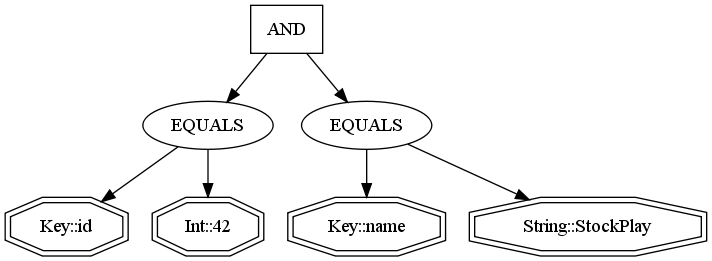
\includegraphics[width=\textwidth]{images/realisatie/AST}
	\caption{Abstract Syntax Tree van een voorbeeldfilter.}
\end{figure}

\section{Verwerking}

Nu de semantiek en conversie van onze filter vastligt, konden we starten met de effectieve implementatie ervan: het omzetten naar of toepassen van de filter op een variabele data-backend. Hierbij zijn de twee grote pistes direct duidelijk: toepassing, of omzetting.

\subsection{Lokale toepassing}

Bij deze opzet wordt de filter lokaal toegepast op een binnengehaalde dataset. Het idee hierbij was om alle records op te halen, en de filter dan lokaal een selectie te laten maken. Die selectie, die voldoet aan de eisen die door de gebruiker zijn opgelegd, kan dan teruggestuurd worden.

Hoewel dit idee perfect toepasbaar is bij systemen waar alle data lokaal aanwezig is (zoals een lokale Java data-backend), treden er problemen op als de data enkel remote aanwezig is en lokaal niet gecachet wordt. In dit geval wordt de overhead van het ophalen van alle records veel te groot, zeker toegepast op StockPlay waarbij de Securities-tabel gemakkelijk meer dan duizend records kan bevatten. Hoewel deze evaluatietechniek dus eenvoudiger te implementeren is (het data-backend-specifieke gedeelte is niet meer aanwezig), hebben we door de grote overhead besloten een alternatief te zoeken.

\subsection{Omzetting}

Het alternatief voor een lokale toepassing, is een omzetting van de filter-boom naar een formaat dat geschikt is om op afstand verwerkt te worden. Hierbij is er geen overhead meer aanwezig, maar wordt het geheel een pak complexer daar het moet kunnen omgezet worden naar een specifieke syntax, afhankelijk van de data-backend.

Om hieraan te kunnen voldoen, hebben we de implementatie van filter sub-objecten (zoals Condities, Relaties, en Data objecten) dusdanig gerealiseerd dat een gemeenschappelijk pseudo-abstract Convertable object (wel instantieerbaar, maar faalt bij aanroepen van de abstracte functies) voorziet in een interface en een set aan functies, terwijl een implementerend object dit gemeenschappelijk object dan moet uitbreiden door de abstracte functies in kwestie in te vullen.

De gemeenschappelijke functionaliteit in dergelijke abstracte objecten voorziet in de verwerking van parameters, het aanbieden van een vaste functie-signatuur, de generatie van een Graph-subtree, en tenslotte in een implementatie van de \emph{compile()} functie. Deze functie, een pijler van de filter-infrastructuur, doet enkele elementaire dingen: het haalt een specifieke Converter op, en het roept diens \emph{process()} functie aan met de gepaste parameters. Een dergelijke Converter -- de implementerende counterpart van het abstract object -- voorziet enkel in een \emph{process()} functie, die opgeroepen wordt wanneer het object gecompileerd wordt.

Deze opzet (pseudo-abstracte Convertable objecten die Converters instanti\"eren) mag misschien complex lijken, maar het is elementair in het generiek maken van de filters. Aangezien de pseudo-abstracte Convertable objecten rechtstreeks instanti\"eerbaar zijn, kan de Parser een boomstructuur aan dergelijke objecten opstellen zonder weet te hebben van hoe die boom uiteindelijk zal gecompileerd worden. Het is slechts wanneer die aanroep effectief gebeurt, dat elk Convertable object zal opvragen hoe hij gecompileerd moet worden, om zo de juiste Converter op te roepen. Die Converters voorzien ook niet in een \emph{compile()} instructie, omdat die instructie geen parameters vastlegt en dus manueel de private dataleden zou moeten raadplegen om parameters op te halen. Om dit te vermijden hebben we gekozen voor een extra instructie, de \emph{process()} instructie, die w\'el voorziet in een specifieke signatuur om zo verkeerde implementaties van de Convertables te vermijden.

\begin{code}
\begin{verbatim}
id = 42 AND name = "StockPlay"
\end{verbatim}
\caption{Finaal resultaat na omzetting door de SQL-converters.}
\end{code}

